\documentclass[output=paper,colorlinks,citecolor=brown]{langscibook}
\author{Robert D. Van Valin, Jr.\orcid{}\affiliation{The State University of New York at Buffalo \& Heinrich Heine University Düsseldorf}}
\title{How language began: A theoretical interpretation}
\abstract{In his book \citew{everett2017language}, Daniel Everett argued that linguistic communication did not originate with \textit{Homo sapiens sapiens} but rather began two million years earlier with \textit{Homo erectus} [\textit{HE}]. The linguistic system proposed by Everett for \textit{HE} is not as complex as modern language but is more than adequate for the demands of \textit{HE}’s sociocultural and technological needs. This paper presents an analysis of the linguistic system of \textit{HE} in terms of a theory of grammar, namely Role and Reference Grammar \citep{van2005exploring}.}


\IfFileExists{../localcommands.tex}{
   \addbibresource{../localbibliography.bib}
   \usepackage{orcidlink}
\usepackage{tabularx,multicol}
\usepackage{url}
\urlstyle{same}

\usepackage{siunitx}
\sisetup{group-digits = none}

\usepackage{langsci-branding} 
\usepackage{langsci-optional}
\usepackage{langsci-lgr}
\usepackage{langsci-tbls}
\usepackage{langsci-gb4e}

% Müller
\usepackage{tikz-qtree}
\usepackage{hologo}

% 3_pullum.tex
\usepackage{langsci-textipa}

% 8_levine
\usepackage{bm}
\usepackage{umoline}
\usepackage{pifont}
\usepackage{pstricks,pst-node,pst-tree}
\usepackage{ulem}
\usepackage{mathrsfs}
\usepackage{bussproofs}

% 14_kornai
\usepackage[matrix,arrow]{xy}
\usepackage{subcaption}

\usepackage[linguistics, edges]{forest}
\usetikzlibrary{arrows, arrows.meta}

   \SetupAffiliations{output in groups = false,
                   orcid placement = after,
                   separator between two = {\bigskip\\},
                   separator between multiple = {\bigskip\\},
                   separator between final two = {\bigskip\\}
                   }

% ORCIDs in langsci-affiliations 
\definecolor{orcidlogocol}{cmyk}{0,0,0,1}
\RenewDocumentCommand{\LinkToORCIDinAffiliations}{ +m }
  {%
    \,\orcidlink{#1}%
  }

\makeatletter
\let\thetitle\@title
\let\theauthor\@author
\makeatother

% Cite and cross-reference other chapters
\newcommand{\crossrefchaptert}[2][]{\citet*[#1]{chapters/#2}, Chapter~\ref{chap-#2} of this volume} 
\newcommand{\crossrefchapterp}[2][]{(\citealp*[#1]{chapters/#2}, Chapter~\ref{chap-#2} of this volume)}
\newcommand{\crossrefchapteralt}[2][]{\citealt*[#1]{chapters/#2}, Chapter~\ref{chap-#2} of this volume}
\newcommand{\crossrefchapteralp}[2][]{\citealp*[#1]{chapters/#2}, Chapter~\ref{chap-#2} of this volume}

\newcommand{\crossrefcitet}[2][]{\citet*[#1]{chapters/#2}} 
\newcommand{\crossrefcitep}[2][]{\citep*[#1]{chapters/#2}}
\newcommand{\crossrefcitealt}[2][]{\citealt*[#1]{chapters/#2}}
\newcommand{\crossrefcitealp}[2][]{\citealp*[#1]{chapters/#2}}


\newcommand{\sub}[1]{\textsubscript{\scriptsize\textrm{#1}}}
% Müller
\newcommand{\page}{}

\let\citew\citet
\def\underRevision{Revise and resubmit}
\let\textbfemph\emph

%% % taken from https://tex.stackexchange.com/a/95079/18561
\newbox\usefulbox

\makeatletter
\def\getslant #1{\strip@pt\fontdimen1 #1}

\def\skoverline #1{\mathchoice
 {{\setbox\usefulbox=\hbox{$\m@th\displaystyle #1$}%
    \dimen@ \getslant\the\textfont\symletters \ht\usefulbox
    \divide\dimen@ \tw@ 
    \kern\dimen@ 
    \overline{\kern-\dimen@ \box\usefulbox\kern\dimen@ }\kern-\dimen@ }}
 {{\setbox\usefulbox=\hbox{$\m@th\textstyle #1$}%
    \dimen@ \getslant\the\textfont\symletters \ht\usefulbox
    \divide\dimen@ \tw@ 
    \kern\dimen@ 
    \overline{\kern-\dimen@ \box\usefulbox\kern\dimen@ }\kern-\dimen@ }}
 {{\setbox\usefulbox=\hbox{$\m@th\scriptstyle #1$}%
    \dimen@ \getslant\the\scriptfont\symletters \ht\usefulbox
    \divide\dimen@ \tw@ 
    \kern\dimen@ 
    \overline{\kern-\dimen@ \box\usefulbox\kern\dimen@ }\kern-\dimen@ }}
 {{\setbox\usefulbox=\hbox{$\m@th\scriptscriptstyle #1$}%
    \dimen@ \getslant\the\scriptscriptfont\symletters \ht\usefulbox
    \divide\dimen@ \tw@ 
    \kern\dimen@ 
    \overline{\kern-\dimen@ \box\usefulbox\kern\dimen@ }\kern-\dimen@ }}%
 {}}
\makeatother

% 1_intro.tex

% For the block quote:
\definecolor{linequote}{RGB}{224,215,188}
\definecolor{backquote}{RGB}{249,245,233}

\NewDocumentEnvironment{myquote}{ +m }
  {%
    \begin{tblsfilled}{}[black!12]
    #1%
  }
  {\end{tblsfilled}}

% 2_gibson.tex


% Example(s) Environments
% 12pt, No new-lines after example number is printed

\newcounter{examplectr}
\newcounter{fnexamplectr}

% Note: don't use subexamples in footnotes.

% This line is to overcome a bug in cmu-art style: it prints counter
% values to the aux file using \theaux... rather than using \the...
\def\theauxexamplectr{\theexamplectr}

\newcounter{subexamplectr}
\def\theauxsubexamplectr{\thesubexamplectr}
\def\theauxfnexamplectr{\thefnexamplectr}

\renewcommand{\theexamplectr}{\arabic{examplectr}}
% This command causes example numbers to appear without following periods

\renewcommand{\thefnexamplectr}{\roman{fnexamplectr}}
% This command causes example numbers to appear without following periods

\renewcommand{\thesubexamplectr}{\theexamplectr\alph{subexamplectr}}
% This command gives the number of an example and subexample as e.g. 1a, 2b

\newlength{\wdth}
\newcommand{\strike}[1]{\settowidth{\wdth}{#1}\rlap{\rule[.5ex]{\wdth}{1pt}}#1}

\newcommand{\exref}[1]{(\ref{#1})}
% This command puts reference numbers with parentheses
% surrounding them 

% The environment ``examples'' gives a list of examples, one on each line,
% numbered with a lower case alphabetic character
\newenvironment{examples}%
   { \vspace{-\baselineskip}
     \begin{list}%
     \textrm{\alph{subexamplectr}.}%
     {\usecounter{subexamplectr}
     \setlength{\topsep}{-\parskip}
     \setlength{\itemsep}{-2pt}
     \setlength{\leftmargin}{0.5in}
     \setlength{\rightmargin}{0in} } }%
   { \end{list}}

% The environment ``myexample'' outputs an arabic counter ``examplectr''
% surrounded by parentheses.
\newenvironment{myexample}
   { \vspace{20pt}
     \noindent
     \begin{minipage}{\textwidth}    % minipage environment disallows
                 % breaks across pages

     \refstepcounter{examplectr}     % step the counter and cause this
                 % section to be referenced by the
                 % counter ``examplectr''
     (\arabic{examplectr})}%
   { \vspace{20pt}
     \end{minipage}}

\newenvironment{myfnexample}
   { \vspace{2pt}
     \noindent
     \begin{minipage}{\textwidth}    % minipage environment disallows
                 % breaks across pages

     \refstepcounter{fnexamplectr}     % step the counter and cause this
                 % section to be referenced by the
                 % counter ``examplectr''
     (\roman{fnexamplectr})}%
   { \vspace{2pt}c
     \end{minipage}}
    
\newcommand*\circled[1]{\tikz[baseline=(char.base)]{
            \node[shape=circle,draw,inner sep=2pt] (char) {#1};}}

\newcommand{\data}[1]{\textit{#1}}
\newcommand{\nodata}[1]{#1}
\newcommand{\blank}{\rule{1.2em}{0.5pt}}
\newcommand{\pt}[1]{\ensuremath{\mathsf{#1}}}
\newcommand{\ptv}[1]{\ensuremath{\textsf{\textsl{#1}}}}
\newcommand{\sv}[1]{\ensuremath{\mathcal{#1}}}

\newcommand{\sX}{\sv{X}}
\newcommand{\sF}{\sv{F}}
\newcommand{\sG}{\sv{G}}
\newcommand{\greekp}{\upvarphi}
\newcommand{\greekr}{\uprho}
\newcommand{\greeks}{\upsigma}
\newcommand{\MultiLine}[1]{\ensuremath{\begin{array}[b]{@{}l@{}}#1\end{array}}}
\newcommand{\LexEnt}[3]{#1; \ensuremath{#2}; \syncat{#3}}

\newcommand{\LexEntBroken}[3]
  {\Shortstack
      {%
        {#1;} 
        {\ensuremath{#2};} 
        {\syncat{#3}}%
      }%
  }

\newcommand{\grey}[1]{\colorbox{mycolor}{#1}}
\definecolor{mycolor}{gray}{0.8}

\newcommand{\gap}{\longrule}
\newcommand{\gp}{\gap}
\newcommand{\vs}{\raisebox{.05em}{\ensuremath{\,\upharpoonright}}}

\newcommand{\E}{ε}

\newcommand{\EBob}[1]{\textsl{#1}}

\newcommand{\B}{\textbf}
\newcommand{\f}{{\color{green}f}}  % Question what does f do? It does not have any output in the
                                % original PDF
%\newcommand{\Lemma}{{\color{pink}Lemma}}
\newcommand{\Lemma}{\ensuremath{\vdots\hskip.5cm\vdots}\noLine}

%\newcommand{\calP}{{\color{pink}calP}} % Sebastian
\newcommand{\calP}{\ensuremath{\mathcal{P}}}


\newcommand{\maru}[1]{\ooalign{\hfil#1\/\hfil\crcr
      \raise.05ex\hbox{\LARGE\mathhexbox20D}}}


%\newcommand{\sem}[2][M\!,g]{\mbox{$[\![ \mathrm{#2} ]\!]^{#1}$}}
\newcommand{\sem}{\ensuremath}

%
\newcommand{\trns}[1]{\textbf{#1}\xspace}
\newcommand{\bs}{{\textbackslash}}
\newcommand{\bsl}{{\bs}}
\newcommand{\fb}[1]{\textsubscript{#1}}
\newcommand{\syncat}[1]{\ensuremath{\mathrm{#1}}}
\newcommand{\term}[1]{\textit{#1}}
\newcommand{\LemmaAlt}{\ensuremath{\vdots\hskip.5cm\vdots}}
\NewDocumentCommand{\VanLabel}{m}{\MakeUppercase{#1}}

   %% hyphenation points for line breaks
%% Normally, automatic hyphenation in LaTeX is very good
%% If a word is mis-hyphenated, add it to this file
%%
%% add information to TeX file before \begin{document} with:
%% %% hyphenation points for line breaks
%% Normally, automatic hyphenation in LaTeX is very good
%% If a word is mis-hyphenated, add it to this file
%%
%% add information to TeX file before \begin{document} with:
%% %% hyphenation points for line breaks
%% Normally, automatic hyphenation in LaTeX is very good
%% If a word is mis-hyphenated, add it to this file
%%
%% add information to TeX file before \begin{document} with:
%% \include{localhyphenation}
\hyphenation{
    Ber-ti-net-to
    caus-a-tive
    fest-schrift
    Fest-schrift
    Hix-kar-ya-na
    In-do-ne-sian
    mor-pho-phon-o-log-i-cal
    Mo-se-tén
    par-a-digm
    phra-ses
    Que-chua
}

\hyphenation{
    Ber-ti-net-to
    caus-a-tive
    fest-schrift
    Fest-schrift
    Hix-kar-ya-na
    In-do-ne-sian
    mor-pho-phon-o-log-i-cal
    Mo-se-tén
    par-a-digm
    phra-ses
    Que-chua
}

\hyphenation{
    Ber-ti-net-to
    caus-a-tive
    fest-schrift
    Fest-schrift
    Hix-kar-ya-na
    In-do-ne-sian
    mor-pho-phon-o-log-i-cal
    Mo-se-tén
    par-a-digm
    phra-ses
    Que-chua
}

   \boolfalse{bookcompile}
   \togglepaper[23]%%chapternumber
}{}

\graphicspath{ {figures/} }

\begin{document}
\maketitle

\section{Introduction: \emph{Homo erectus} and language: A long-standing puzzle}
While full-blown language is generally agreed to be a property of \emph{Homo sapiens sapiens}, there is tantalizing evidence that points to earlier humans as having some kind of communication system much more sophisticated than animal systems yet not as complex as modern language. \citet{everett2017language} makes the case for human language to have originated well before the advent of \emph{Homo sapiens sapiens}, some two million years earlier with \emph{Homo erectus}. Unlike the risible Prometheus story invented by Chomsky, there are solid grounds for concluding that Upright Man had a communication system which was much more sophisticated than animal call systems, if not as complex as modern language.  Everett reviews these in detail and presents convincing evidence for this view.  One strong piece of evidence is the geographical distribution of \emph{Homo erectus}: groups migrated out of Africa not only into Europe and the Middle East but all the way to Southeast Asia and China.  So-called “Peking Man” was \emph{Homo erectus}, as was “Java Man”.  The trek into Southeast Asia involved crossing substantial bodies of water, and this required building and operating watercraft.  It is inconceivable that such journeys could be accomplished by groups with no way to convey complex thoughts and ideas among themselves, especially when it came to building and operating watercraft.  

The discussion will proceed as follows. The first section introduces the complexity hierarchy of grammars assumed by Everett.  The second section presents a sketch of a Role and Reference Grammar [RRG] \citep{van2005exploring,van1997syntax} analysis of the system which \emph{Homo erectus} might have utilized.  The third section concerns the role of information structure in communication systems as simple as these and the implications for conclusions about \emph{Homo erectus}.  The fourth section briefly touches on how a system like that of \emph{Homo erectus} could have evolved into a grammar higher on the hierarchy of grammars introduced in \sectref{sec:vanvalin:2}. Conclusions follow in \sectref{sec:vanvalin:6}.

The analysis to be presented is agnostic with respect to whether the communication system attributed to \emph{Homo erectus} was manual or oral or some combination of the two modalities.

\section{Complexity of grammars: Everett’s hierarchy}\label{sec:vanvalin:2}
One of the immediate difficulties in discussing the possible linguistic abilities of early humans is the obvious fact that they are very different from those of modern humans, and accordingly, if the question is phrased “did early humans have language?”, where “language” is understood as being like contemporary linguistic systems, the answer is obviously “no”.  Everett avoids this trap by talking instead of grammars and proposing a hierarchy of grammars in terms of their formal complexity: $G_3 \Rightarrow G_2 \Rightarrow G_1$.  The simplest grammar, $G_1$, is dubbed a “linear grammar” by Everett, because it permits only sequences of expressions without any embedding of one expression in another. An example is given in \REF{vanvalin_example_1}.

\ea \label{vanvalin_example_1}
Output of a $G_1$ linear grammar: “Man see deer \ldots{}  Deer big \ldots{}  Man spear deer \ldots”\footnote{It is irrelevant for this discussion whether the word order is Actor-\textsc{pred}-Undergoer, Actor-Undergoer-\textsc{pred}, or \textsc{pred}-Actor-Undergoer.}
\z

Each of the expressions is a simple proposition, which may be juxtaposed linearly with other simple propositions to form more semantically complex utterances.

The intermediate grammar in the hierarchy, $G_2$, is labeled a “hierarchical grammar”, because it allows the embedding of one expression inside another, e.g. a modifier inside of a reference phrase.  This is exemplified in \REF{vanvalin_example_2}.

\ea \label{vanvalin_example_2}
Output of a $G_2$ hierarchical grammar: “Man see big deer \ldots{}  He spear it \ldots”
\z

Instead of having a separate proposition \emph{deer big}, the information regarding the size of the deer is incorporated into the referring expression \emph{deer}.

$G_3$ is a “recursive hierarchical grammar”, the complex grammatical system characteristic of most, but not necessarily all, modern languages.  Everett suggests that most likely \emph{Homo erectus} had a $G_1$ grammar, and that will be the focus of this discussion.

\section{A Role and Reference Grammar analysis of $G_1$ grammars}\label{sec:vanvalin:3}

On p. 198 of \citew{everett2017language} there is a partial RRG tree diagram illustrating some of the structural complexity in a $G_3$ grammar.  That tree represents only one of the four projections of the clause posited in RRG: there are constituent, operator, information structure, and prosodic projections. Only the first two are represented in \figref{fig:fig1} below.  

The constituent projection contains lexical items functioning as predicators, arguments, adjuncts and modifiers.  The layered structure of the clause consists of the \textsc{nucleus}, the syntactic unit housing the predicating element, typically, but not necessarily, a verb.  The nucleus plus the semantic arguments of the predicator constitute the \textsc{core} of the clause.  The English verb \textit{give} has three semantic arguments, yet there are only two arguments in the core in \figref{fig:fig1}. The third semantic argument is a WH-expression, and occurs displaced in the \textsc{pre-core slot}, the normal position for displaced WH-expressions in many languages. Locative and temporal adjuncts normally appear in the core-level periphery, since they specify where and when the event coded in the core takes place.  In this example the temporal adjunct \textit{yesterday} functions as a frame-setting topic and occurs in the \textsc{pre-detached position}.  The \textsc{clause} contains the core plus the \textsc{pre-core slot} and the core-level periphery, while the \textsc{sentence} includes the clause, the clause-level periphery, and the pre-detached position.\footnote{Some languages have a  \textsc{post-core slot} and/or a \textsc{post-detached position}.}

\begin{figure}
\centering
\includegraphics[width=0.8\textwidth]{vanvalin_figure1.png}
\fittable{%
\begin{forest}
  [SENTENCE,calign=child, calign child=2
   [PrDP, tier=core
      [ADV, tier=v
         [Yesterday, tier=word]
      ]
   ]
   [CLAUSE, name=clause1,calign=child, calign child=2
      [PrCS, tier=core
         [RP, tier=v
            [~, text width=1cm, tier=word, no edge]
            [what, text width=1cm, tier=word]
            [did, text width=1cm, tier=word, no edge, name=did]
         ]
      ]
      [CORE, name=core, tier=core
         [RP, text width=1cm, text centered
            [John, tier=word]
         ]
         [NUC, text width=1cm, text centered
            [PRED
               [V, tier=v
                  [give, tier=word
                     [\textsc{nuc},s=-5mm
                        [\textsc{core}
                           [\textsc{clause}, name=clause2
                              [\textsc{clause}, name=clause3
                                 [\textsc{sentence}
                              ]
                           ]
                        ]
                     ]
                  ]
               ]
            ]
            ]
         ]
         [PP, text width=1cm, text centered
            [to Mary, tier=word]
         ]
   ]
      [PERIPHERY, name=periphery, tier=core, no edge
         [PP, tier=v
            [in the library?, tier=word]
         ]
      ]
   [~, tier=core, no edge]
  ]
   [~, tier=core, no edge]
]
\node(TNS)[left=0.5cm of clause2]{\textsc{tns}};
\node(IF)[left=1cm of clause3]{\textsc{if}};
\node(cp)[left=9cm of clause1]{\textbf{Constituent projection}};
\node[below=9.5cm of cp]{\textbf{Operator projection}};
\draw[dotted,thick](did.south)--(TNS);
\draw[dotted,thick](did.south)--(IF);
\draw[->](TNS)--(clause2);
\draw[->](IF)--(clause3);
\draw[->](periphery)--(core);
\end{forest}
}

\caption{\label{fig:fig1}Clause structure in a $G_3$ language}
\end{figure}


The auxiliary \emph{did} is not attached to the constituent projection, because it is not lexical but  rather grammatical in nature: it expresses two important operators, tense and illocutionary force.  It is, therefore, attached to the operator projection.

What would a sequence of utterances in a $G_1$ language look like?  Consider the following mini discourse in \REF{vanvalin_example_3}.

\ea \label{vanvalin_example_3}Near river \ldots{}  I see deer \ldots{}  (It/deer) big \ldots{}  (I) spear (it/deer) \ldots\z
It would have the following structure.
\begin{figure}
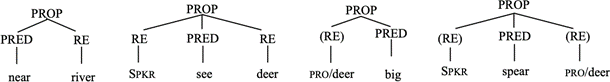
\includegraphics[width=\textwidth]{vanvalin_figure2.png}
\caption{\label{fig:fig2}Structure of utterances in $G_1$ language}
\end{figure}

The first thing to note is the lack of syntactic categories.  There are no grounds for attributing syntactic categories or syntactic structure to these utterances.  The categories are all semantic: ‘\textsc{re}’ is \textsc{referring expression} and is not phrasal; ‘\textsc{pred}’ is \textsc{predicator}; and ‘\textsc{prop}’ is \textsc{proposition}.  A proposition consists of a predicator and its arguments. There are no adjuncts modifying the proposition or any of its constituents.  When a location needs to be mentioned, for example, it is expressed as an independent locative proposition, analogous to the independent attributive proposition involving the referring expression \emph{deer}.  

The equivalent of lexical modifiers, as illustrated in \figref{fig:fig2}, would be represented as independent propositions.  What about non-lexical, i.e. grammatical, modifiers?  It is highly unlikely that there are any grammatical modifiers of this kind found in a $G_1$ grammar of the type posited for \emph{Homo erectus}.  Hence there would not be an operator projection in the representation of utterances.  However, there are two operators which are found in the grammar of every $G_2$ and $G_3$ human language and must have been part of any possible \emph{Homo erectus} $G_1$ system: negation and illocutionary force. Negation is essential for reasoning as well as for important speech acts like negative imperatives and warnings.  The ability to make assertions, ask questions and give commands is an essential part of any human communication system.  It is for these reasons that RRG claims that negation and illocutionary force are the only universal operators.  Both can be expressed through non-grammatical means: illocutionary force can be signaled prosodically, while negation can be expressed gesturally.  Hence they would not motivate an operator projection in the structures.

\section{Information structure, argument realization, and cooperation}\label{sec:vanvalin:4}

In the hypothetical $G_1$ example in \REF{vanvalin_example_3} and \figref{fig:fig2}, after the first mention of a referent, there are three possibilities for subsequent mentions: (1) repetition of the referring expression, (2) using a \textsc{pro} form, or  (3) simple omission, as is often the case in many $G_3$ languages today.  Option 1 requires no special machinery; it is the most redundant.  Option 2 is the least likely, since the development of \textsc{pro} forms seems to be more likely a trait of the advanced systems.  The most interesting option is (3).  It was argued in \citet{van1990functionalism} and \citet{van1997syntax}, following Kuno, Bolinger and Bickerton, that information structure plays a central role in the analysis of intrasentential pronominalization, regardless as to whether it involves overt \textsc{pro} forms or zero anaphora.  For example, a referent cannot be realized as zero if it is part of the actual focus 
domain of the clause but can be if it is part of the background.  So in the earlier example, it would be nonsensical to introduce \emph{the deer} using zero coding.  Hence overt occurrence vs. omission would likely not be beyond the means of \emph{Homo erectus}.  Thus possibility (3) is very much an option.

If \emph{Homo erectus} is sensitive to some aspects of information structure, then this has significant consequences for the issues raised at the outset of this discussion.  It was argued in \citet{van1993synopsis}, following \citet{kempson1975presupposition}, that the notions of topic and focus, which are fundamental to information structure, are ultimately derived from Grice’s Cooperative Principle and the maxim of quantity, which are general (i.e. not domain-specific) rational principles of human behavior.  Cooperation is a hallmark of language users, and despite the fact that it is certain that \emph{Homo erectus} did not wield the Cooperative Principle in the same way as modern $G_3$ language users do, it nevertheless was a necessary part of \emph{Homo erectus} cognition.  An example where cooperation would be vital is trying to reach islands separated from them by a significant body of water; cooperation is essential in the construction and operation of the primitive watercraft on which they traveled and on which their lives depended.

\section{The transition from $G_1$ to $G_2$}\label{sec:vanvalin:5}

A $G_2$ grammar would differ from a $G_1$ grammar in significant ways.  To begin with, the combination of adjunct modifiers and referring expressions yields \textsc{reference phrases}, which are necessarily syntactic, because a reference phrase potentially consists of two or more units that are not of the same semantic type, e.g. [$_{RP}$ [$_{PRED}$ big] → [$_{RE}$ deer] ].  In the same vein, the coocurrence of syntactic reference phrases in a proposition triggers a reanalysis of the proposition as a syntactic entity, a core.  In addition, the occurrence of adjunct modifiers taking a propositional unit as an argument, e.g. \textit{I see big deer near river} (i.e. \textbf{near}´ (river, [\textsc{spkr} see big deer])), further motivated the reanalysis, as the predicate+argument(s) unit is now functioning as an argument and filling a slot that could also be filled by a syntactic entity, namely a reference phrase (e.g. \textit{Big deer near river}).  The predicator underwent reanalysis as a syntactic nucleus due to, among other things, the occurrence of syntactic entities as the predicator, e.g. ‘\textsc{spkr} good hunter’.  Thus, the introduction of embedding had profound implications, because it created semantically mixed units which led to the reanalysis of the fundamental semantic entities as syntactic, as illustrated in \figref{fig:fig3}.

\begin{figure}
\centering
\includegraphics[width=0.8\textwidth]{vanvalin_figure3.png}
\caption{\label{fig:fig3}The transition from $G_1$ to $G_2$}
\end{figure}

The two most salient changes are the transformation of the attributive predicator \textit{big} into a part of the referring expression \emph{deer}, thereby creating a syntactic reference phrase, and the reanalysis of the locative proposition \emph{by the river} into a propositional modifier.  The result is more compact expressions with modification relations directly coded.  

\section{Conclusion}\label{sec:vanvalin:6}
In this brief note I have sketched out what an RRG analysis of a $G_1$ linguistic system which could have been employed by \emph{Homo erectus} might have looked like, based on the account given in \citet{everett2017language}.  Dubbed a “linear grammar” by Everett, it would specify a linear string of propositions, as in \figref{fig:fig2}, which would be semantic in nature.  There is nothing to motivate the positing of syntactic categories or structure.  Of particular interest is the role of information structure, which gives evidence that Upright Man had a rudimentary understanding of Grice’s Cooperative Principle and at least the the maxim of quantity, since it underlies the important notions of topic and focus.  

There is little agreement among researchers investigating primate cognition as to whether non-human primates have shared intentionality, i.e. the ability to recognize con-specifics as being intentional and mental agents.  It is clear, however, that early humans, including \emph{Homo erectus}, had shared intentionality.  They were, so to speak, “Gricean apes”.

The transition from a semantic $G_1$ to a syntactic $G_2$ was briefly discussed.  It was argued that the introduction of embedding into the grammar led to a transformation of the grammar from being essentially semantic to being primarily syntactic.

Thus, Everett’s proposals regarding the linguistic abilities of \emph{Homo erectus} together with the well-motivated theoretical constructs of RRG yield important insights into how language began.

\section*{Abbreviations}
\begin{tabularx}{.5\textwidth}{@{}lQ@{}}
\textsc{if} & illocutionary force \\
\textsc{nuc} & nucleus \\
\textsc{p}r\textsc{cs} & pre-core slot \\
\textsc{p}r\textsc{dp} & pre-detached position \\
\textsc{pred} & predicator \\
\textsc{prop} & propositional \\
\textsc{re} & referring expression \\
\textsc{rp} & reference phrase \\
\textsc{spkr} & speaker \\
\textsc{tns} & tense \\
\end{tabularx}

\printbibliography[heading=subbibliography,notkeyword=this]
\end{document}
